\sloppy
\chapter{Proposed Approach}
\addtocontents{toc}{\protect\setcounter{tocdepth}{2}}
\section{Introduction}

This chapter describes the fake news detection system proposed and evaluated in this thesis. It starts with a formal problem statement and presents the system model as an end-to-end pipeline. It then describes the BERT + BiLSTM classification architecture and its algorithm, and closes with the reasons for combining a transformer encoder with a sequential BiLSTM layer.

\section{Problem Statement}

Given a news text $T$ (an article body, a headline, or a short statement), the goal is to learn a classification function $f(T) \rightarrow \{\text{REAL}, \text{FAKE}\}$ that predicts whether $T$ is genuine or fabricated or misleading, together with a confidence score. The function $f$ is learned from labelled training data drawn from one or more benchmark datasets. It must generalize to unseen examples from the same dataset and, ideally, across datasets that differ in source, writing style, and label distribution. This thesis tests that ability on LIAR and ISOT, as described in Chapter~4.

The thesis investigates three candidate realizations of $f$: a purely sequential deep learning model (BiLSTM), a purely transformer-based model (BERT), and a hybrid that composes both (BERT + BiLSTM). The aim is to determine empirically which one gives the best trade-off between detection accuracy, generalization across datasets, and model complexity.

\section{System Model}

The proposed system is a multi-stage pipeline that turns unstructured news input into a classification with a confidence estimate. Figure~\ref{fig:systemmodel} shows the overall architecture.

\begin{figure}[H]
    \centering
    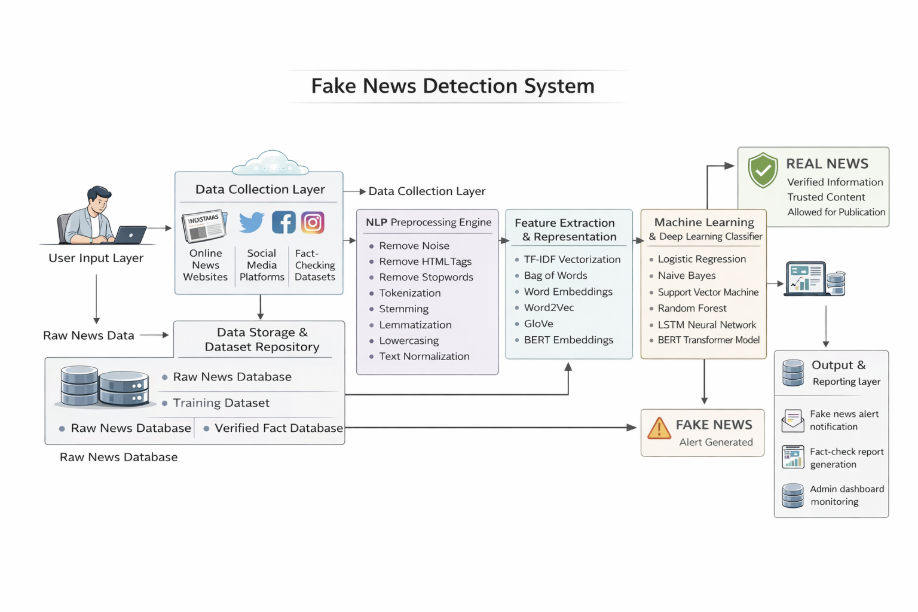
\includegraphics[width=0.95\textwidth]{./chap4-proposedapproach/architecture.png}
    \caption{End-to-end fake news detection system pipeline, from user input through data collection, NLP preprocessing, feature extraction, classification, and output reporting}
    \label{fig:systemmodel}
\end{figure}

The pipeline has the following stages:

\begin{itemize}
\item \textbf{User Input Layer:} Accepts raw news input as free text, a headline, or a URL pointing to a news article.
\item \textbf{Data Collection Layer:} Gathers data from the benchmark datasets (LIAR, ISOT, FakeNewsNet) and, where applicable, from online news websites, social media platforms, and fact-checking sources.
\item \textbf{Data Storage and Dataset Repository:} Stores raw news data, training, validation, and test splits, and verified fact databases for reuse across experiments.
\item \textbf{NLP Preprocessing Engine:} Cleans and normalizes the raw text by removing noise and HTML tags, removing stopwords, tokenizing, stemming, lemmatizing, and lowercasing.
\item \textbf{Feature Extraction and Representation Layer:} Converts the normalized text into numeric representations with TF-IDF, Bag-of-Words, Word2Vec, GloVe, or BERT embeddings, depending on the downstream classifier.
\item \textbf{Machine Learning and Deep Learning Classifier:} Hosts the candidate models compared in this thesis (BiLSTM, BERT, and the hybrid BERT + BiLSTM) and produces a REAL or FAKE prediction with a confidence score.
\item \textbf{Output and Reporting Layer:} Returns the final decision with a human-readable report that can feed a fake-news alert, a fact-check report, or an administrative monitoring dashboard.
\end{itemize}

The layered design keeps preprocessing, representation, and modelling separate, so the classifiers evaluated in Chapter~4 (BiLSTM, BERT, BERT + BiLSTM) can be swapped without changing the rest of the pipeline.

\section{Proposed BERT + BiLSTM Detection Framework}

Figure~\ref{fig:systemmodel} shows the pipeline at a high level. Figure~\ref{fig:architecture} shows the architecture of the hybrid BERT + BiLSTM classifier in detail.

\begin{figure}[H]
    \centering
    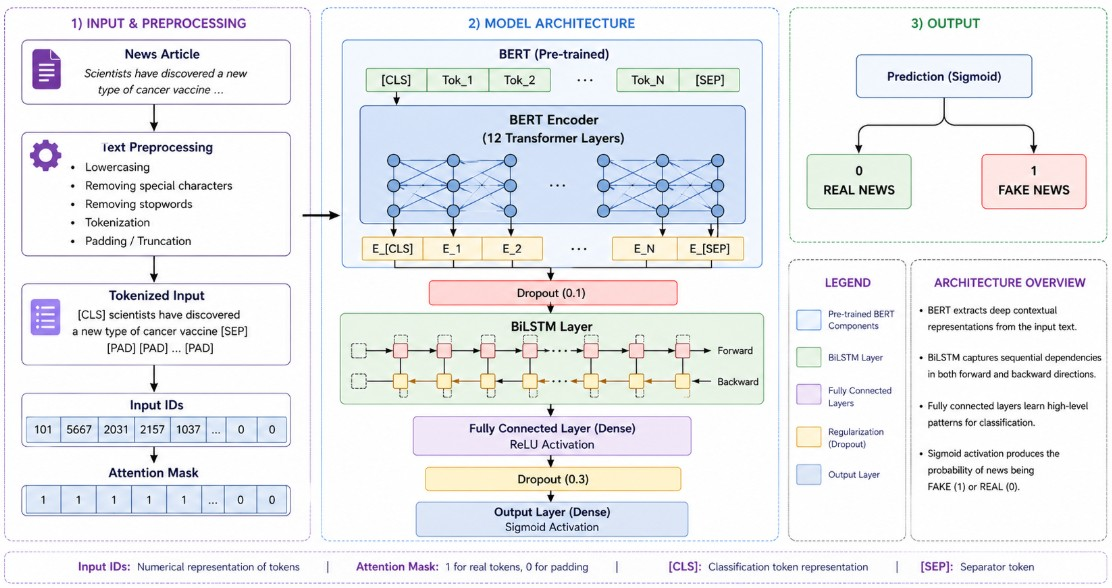
\includegraphics[scale=0.6]{./chap4-proposedapproach/Arch.jpg}
    \caption{Detailed architecture of the proposed BERT + BiLSTM fake news detection model}
    \label{fig:architecture}
\end{figure}

The input article is first tokenized and normalized (lowercasing, special-character removal, stopword removal, tokenization, padding or truncation). This yields a fixed-length sequence of token IDs and an attention mask. The sequence, prefixed with a \texttt{[CLS]} token and suffixed with a \texttt{[SEP]} token, passes through a pre-trained BERT encoder of 12 Transformer layers. The encoder produces a contextual embedding for every token position ($E_{[CLS]}, E_1, \ldots, E_N, E_{[SEP]}$).

Simple BERT fine-tuning keeps only the \texttt{[CLS]} embedding. The proposed model instead passes the whole sequence of contextual embeddings through a dropout layer (rate 0.1) and into a BiLSTM layer. The BiLSTM reads the sequence forward and backward to capture sequential dependencies over BERT's already contextualized representations. Its output goes through a fully connected layer with ReLU activation and a second dropout layer (rate 0.3). A final dense layer with sigmoid activation outputs the probability that the input is fake (1) or real (0).

\subsection{Proposed Algorithm}

Algorithm~\ref{alg:bertbilstm} summarizes the classification procedure of the BERT + BiLSTM model.

\begin{algorithm}[H]
\SetAlgoLined
\KwIn{Raw news text $T$}
\KwOut{Classification label $y \in \{\text{REAL}, \text{FAKE}\}$ with confidence score}
Preprocess $T$: apply noise removal, lowercasing, tokenization, stopword removal, and lemmatization\;
Tokenize the preprocessed text using BERT's WordPiece tokenizer, prepend \texttt{[CLS]} and append \texttt{[SEP]}\;
Pass the tokenized sequence through the pre-trained BERT encoder to obtain contextual embeddings $E_{[CLS]}, E_1, \ldots, E_N, E_{[SEP]}$\;
Apply dropout to the sequence of contextual embeddings\;
Pass the embedding sequence through a BiLSTM layer to obtain sequence-aware hidden representations\;
Pass the BiLSTM output through a fully connected layer with ReLU activation\;
Apply dropout, then pass the result through an output dense layer with sigmoid activation\;
\Return{predicted label $y$ (REAL or FAKE) and its associated confidence score}\;
\caption{Fake News Detection using the Proposed BERT + BiLSTM Model}
\label{alg:bertbilstm}
\end{algorithm}

\subsection{Design Rationale: Why Combine BERT and BiLSTM?}

The reason for combining BERT and BiLSTM is not that BiLSTM performs poorly alone, although it does under the training conditions used in this thesis (Chapter~4). The two model families have complementary strengths. BERT captures context and semantics through its bidirectional Transformer design and self-attention, but it aggregates sequence-level information through attention and not through explicit sequence modelling of the kind recurrent networks perform.

BiLSTM is built to model sequences and positional dependencies, and it reads its input in both directions. In the hybrid, BERT acts as a contextual feature extractor that produces informative token-level embeddings. Instead of depending only on the \texttt{[CLS]} token, the whole sequence of embeddings goes into the BiLSTM, which adds explicit sequential modelling on top of BERT's contextual representations.

The hybrid is therefore designed to benefit from both contextual embeddings and sequential learning. Whether this complementarity gives a measurable accuracy gain in practice, and under what training conditions, is examined in Chapter~4.

\section{Summary}

This chapter presented the proposed system: a formal problem statement, an end-to-end pipeline from input collection through NLP preprocessing, feature extraction, classification, and reporting, and the BERT + BiLSTM architecture with its algorithm and design rationale. Chapter~4 evaluates this model together with the standalone BiLSTM and BERT baselines on several benchmark datasets.
